\section{Complete System Overview}
%
\subsection{Interactions and Responsibilites}
The theme class is implemented as flyweight, holding references to previously 
created instances of a particular theme. If a requested theme type is not yet 
held in the list of instances, the class calls a builder class, 
FBThemeBuilder~\ref{fig:system}, to parse the requested theme's XML file, 
load the images and then return a fresh instance of the theme. Additionally, 
each theme contains an FBImageLibrary. The image library is just a simple 
wrapper around an IdentityDictionary to ease filling it with Forms. 
FBTheme and FBImageLibrary also support scaling to adjust to any screen 
size (without accounting for neccessary interpolation).
%
\begin{figure}[bt]
  \begin{center}
%    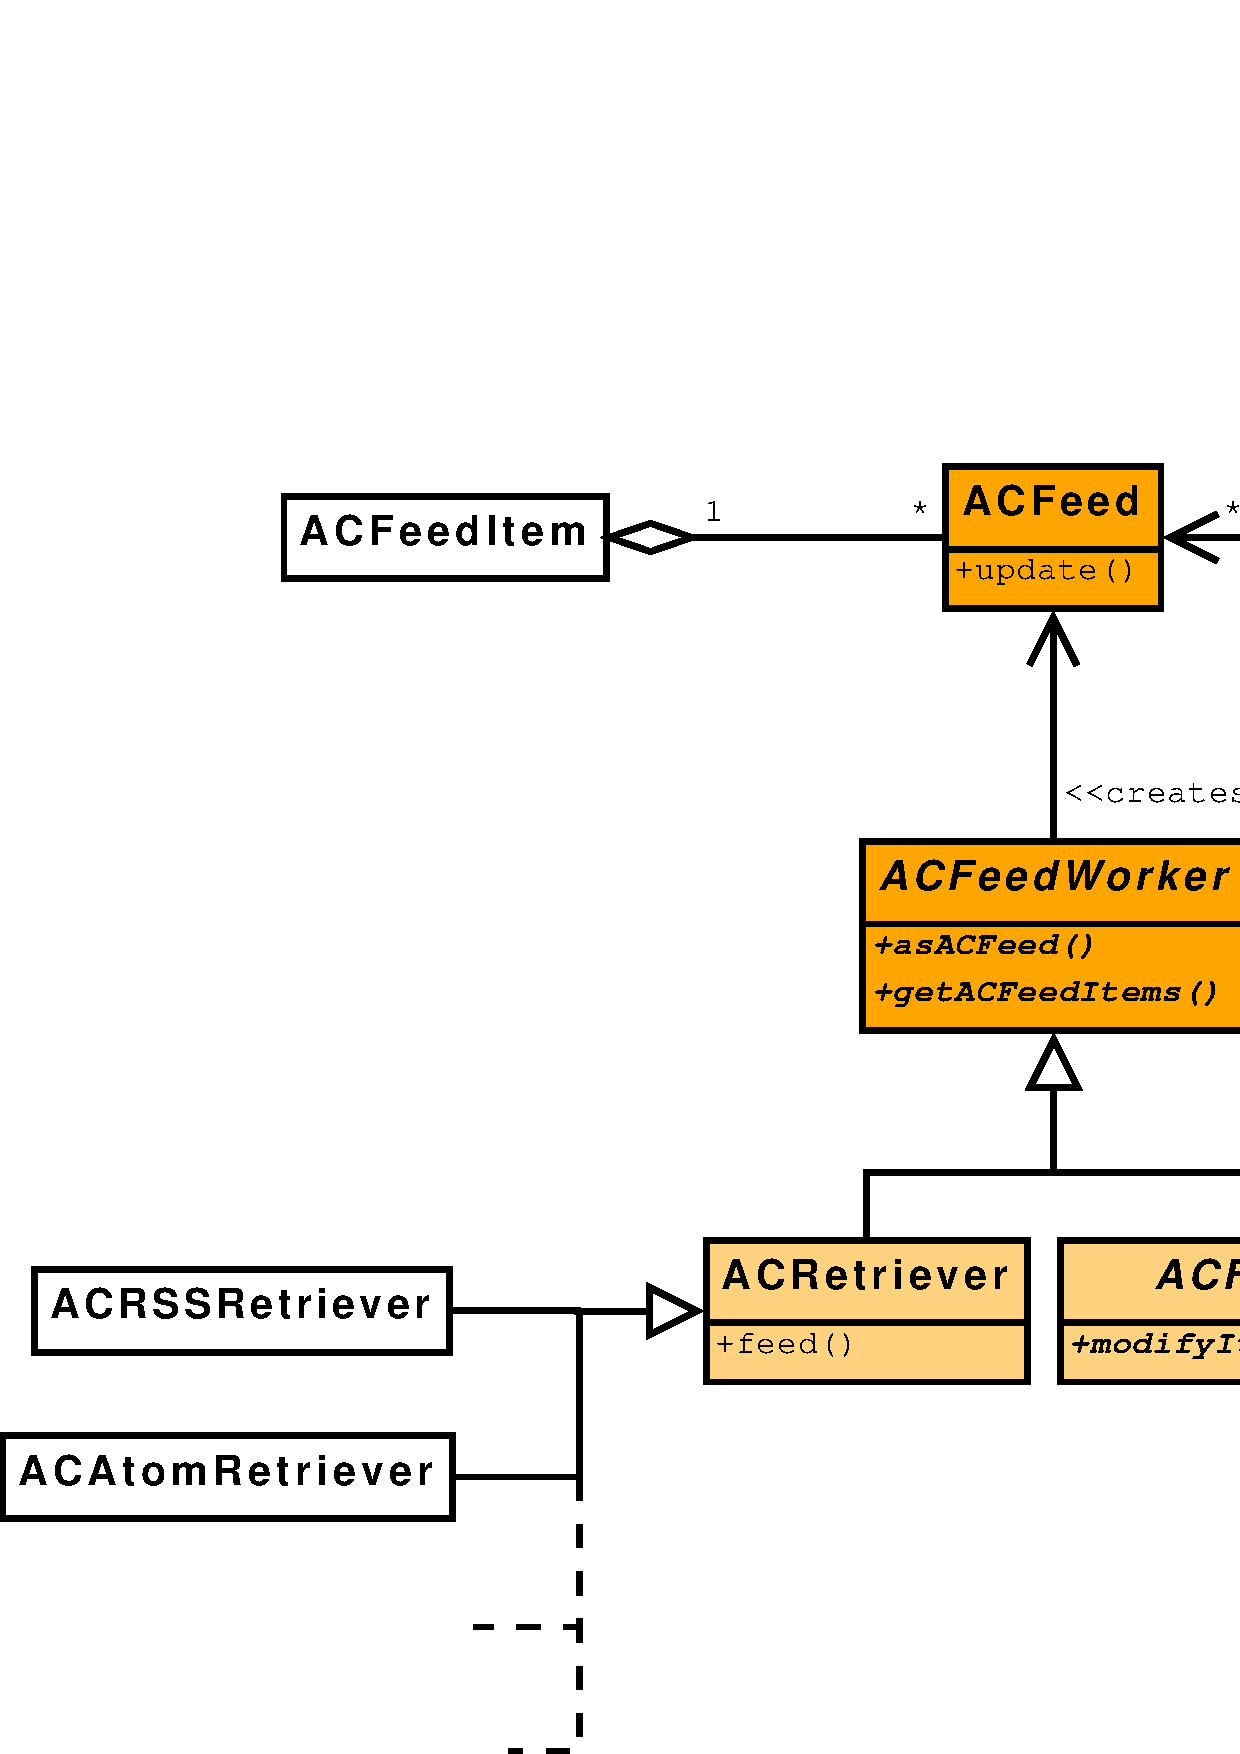
\includegraphics[width=0.9\linewidth]{images/system.png}
  \end{center}
  \caption{The complete system overview}
  \label{fig:system}
\end{figure}
%
There are a couple of supporting classes which add to the game logic 
in Fig.\ref{fig:system}(1). Those implement different strategies for 
rewarding the player for good gaming. Good gaming is correlated to the 
number of balls falling, if more are falling at the same time, more 
reward points are gained.
The reward strategies implement a method
rewardPlayer:for:~\ref{lst:reward}.\\
In single player mode, a
simple highscore is added to the screen (responsible for adding the 
score visual is also the strategy itself) and for any number of 
reward points reported by the FBPlayfield, points are added to the 
score. 
%
\begin{figure}
  \begin{center}
    \begin{lstlisting}
rewardPlayer: aPlayer for: anAchievmentScalar
    "I reward a single player with an exponentially 
rising rate of points" 

    self score:
         self score + (anAchievmentScalar raisedTo: 2)
    \end{lstlisting}
  \end{center}
  \caption{The highscore calculation method}
  \label{lst:reward}
\end{figure}
In multiplayer mode, the reward only applies, if the player eliminates 
more than three balls from the field with a single shot. If that happens, 
a number of balls half as great is distributed among the other players,
and shot randomly in any direction. This happens via a call to 
the playfields who have to shoot random balls, since FBRewardStretegies
hold a collection referring to all playfields.

As aforementioned, FBPlayfield is responsible for creating its own 
contents~\ref{fig:system}(2). Such content displays a cannon, a 
player avatar , messages for the user and numerous coloured balls. 
Each of these serves only a single, limited purpose, with FBPlayer 
and FBMessage merely wrapping different types of graphical response.
The cannon is the entity that reacts to the user's input, panning 
left and right and sending balls off into the field. However, it 
is controlled entirely by the playfield and does not act itself.

The FBBall is an exception to this simplicity. 
\begin{description}
  \item[First]
    	it has to look 
	differently, showing different colors in our themes. 
  \item[Secondly]
    	a Ball has different stages in its lifetime, being 
	loaded into the cannon, then flying, hanging from the 
	ceiling (or, indeed, from other balls) and finally falling 
	and vanishing.
  \item[Finally]
    	a Ball needs to collide with the playfield boundaries and 
	other balls in the field.
\end{description}
%
Thus its implementation is a bit larger, as it implements the FBCollider 
interface, utilizes different ``states'' to act on in its step method and 
and also draws itself from a collection of images.
%
\subsection{Ball Collisions}
%
\subsection{Falling Balls}
%
When a ball collides with another and gets stuck, the playfield asks the 
collision map whether this connects three or more balls of the same color.
If so, those balls are requested to fall down.\\
However, if other balls are hanging off those balls which are falling, 
they will have to fall down to, with nothing to hold them. We looked 
into several ways of checking for such conditions, like regarding balls in the 
playfield as a network of nodes, using a graph search algorithm to determine 
whether or not a given ball is connected to the top of the playfield via 
others. This proved difficult to implement and hurting encapsulation. Thus 
we applied a metaphor of a garbage collector (GC) to the problem. First we used a
reference counting GC where each ball registered itself with the balls he hung 
off. If those balls fell, they reported to each registree so that those would 
decrement their reference count. If the reference count fell to zero, the ball 
would fall. However, this approach led to some problems with circular shapes 
in the playfield. Due to this we switched to a mark and sweep GC which iterates 
over the balls in the field. Though this might sound less optimal performance-wise,
you have to keep in mind that the number of balls in one playfield is relatively limited, 
and also that the GC runs at a moment where the user cannot shoot anyway, so 
it is not time-critical.

